\documentclass{beamer}

%
% Choose how your presentation looks.
%
% For more themes, color themes and font themes, see:
% http://deic.uab.es/~iblanes/beamer_gallery/index_by_theme.html
%
\mode<presentation>
{
  \usetheme{default}      % or try Darmstadt, Madrid, Warsaw, ...
  \usecolortheme{default} % or try albatross, beaver, crane, ...
  \usefonttheme{default}  % or try serif, structurebold, ...
  \setbeamertemplate{navigation symbols}{}
  \setbeamertemplate{caption}[numbered]
  \setbeamertemplate{footline}[page number]
  \setbeamercolor{frametitle}{fg=white}
  \setbeamercolor{footline}{fg=black}
} 

\usepackage[english]{babel}
\usepackage[utf8x]{inputenc}
\usepackage{tikz}
\usepackage{listings}
\usepackage{courier}

\xdefinecolor{darkblue}{rgb}{0.1,0.1,0.7}
\xdefinecolor{dianablue}{rgb}{0.18,0.24,0.31}
\definecolor{commentgreen}{rgb}{0,0.6,0}
\definecolor{stringmauve}{rgb}{0.58,0,0.82}

\lstset{ %
  backgroundcolor=\color{white},      % choose the background color
  basicstyle=\ttfamily\small,         % size of fonts used for the code
  breaklines=true,                    % automatic line breaking only at whitespace
  captionpos=b,                       % sets the caption-position to bottom
  commentstyle=\color{commentgreen},  % comment style
  escapeinside={\%*}{*)},             % if you want to add LaTeX within your code
  keywordstyle=\color{blue},          % keyword style
  stringstyle=\color{stringmauve},    % string literal style
  showstringspaces=false,
  showlines=true
}

\lstdefinelanguage{scala}{
  morekeywords={abstract,case,catch,class,def,%
    do,else,extends,false,final,finally,%
    for,if,implicit,import,match,mixin,%
    new,null,object,override,package,%
    private,protected,requires,return,sealed,%
    super,this,throw,trait,true,try,%
    type,val,var,while,with,yield},
  otherkeywords={=>,<-,<\%,<:,>:,\#,@},
  sensitive=true,
  morecomment=[l]{//},
  morecomment=[n]{/*}{*/},
  morestring=[b]",
  morestring=[b]',
  morestring=[b]"""
}

\title[2016-05-19-uscms-diana]{The DIANA-HEP Project}
\author{Jim Pivarski}
\institute{Princeton University -- DIANA}
\date{May 19, 2016}

\begin{document}

\logo{\pgfputat{\pgfxy(0.11, 8)}{\pgfbox[right,base]{\tikz{\filldraw[fill=dianablue, draw=none] (0 cm, 0 cm) rectangle (50 cm, 1 cm);}}}\pgfputat{\pgfxy(0.11, -0.6)}{\pgfbox[right,base]{\tikz{\filldraw[fill=dianablue, draw=none] (0 cm, 0 cm) rectangle (50 cm, 1 cm);}
\includegraphics[height=0.99 cm]{diana-hep-logo.png}\tikz{\filldraw[fill=dianablue, draw=none] (0 cm, 0 cm) rectangle (4.9 cm, 1 cm);}}}}

\begin{frame}
  \titlepage
\end{frame}

\logo{\pgfputat{\pgfxy(0.11, 8)}{\pgfbox[right,base]{\tikz{\filldraw[fill=dianablue, draw=none] (0 cm, 0 cm) rectangle (50 cm, 1 cm);}
\includegraphics[height=1 cm]{diana-hep-logo.png}}}}

% Uncomment these lines for an automatically generated outline.
%\begin{frame}{Outline}
%  \tableofcontents
%\end{frame}

\begin{frame}{Principle Investigators}
\scriptsize

\vfill

\begin{columns}[t]
\column{0.5\linewidth}
\textcolor{darkblue}{Peter Elmer (Princeton)}
\begin{columns}
\column{0.25\linewidth}
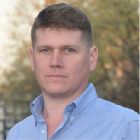
\includegraphics[height=2 cm]{peter_elmer.png}
\column{0.75\linewidth}
\begin{itemize}
\item Many roles in Software/Computing in BaBar and CMS
\item Early involvement in xrootd, etc.
\end{itemize}
\end{columns}

\column{0.5\linewidth}
\textcolor{darkblue}{Mike Sokoloff (Cincinnati)}
\begin{columns}
\column{0.25\linewidth}
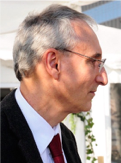
\includegraphics[height=2 cm]{mike_sokoloff.png}
\column{0.75\linewidth}
\begin{itemize}
\item Flavor analysis on BaBar/LHCb
\item NSF-funded R\&D investigation into many/multicore: GooFit prototype, likelihood fitting
\end{itemize}
\end{columns}
\end{columns}

\vfill
\begin{columns}[t]
\column{0.5\linewidth}
\textcolor{darkblue}{Brian Bockelman (Nebraska-Lincoln)}
\begin{columns}
\column{0.25\linewidth}
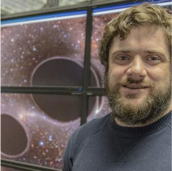
\includegraphics[height=2 cm]{brian_bockelman.png}
\column{0.75\linewidth}
\begin{itemize}
\item Computer Science research faculty
\item CMS and Tier2 Computing and Open Science Grid
\item NSF-funded AAA project (xrootd-based data federation)
\item I/O performance research
\end{itemize}
\end{columns}

\column{0.5\linewidth}
\textcolor{darkblue}{Kyle Cranmer (NYU)}
\begin{columns}
\column{0.25\linewidth}
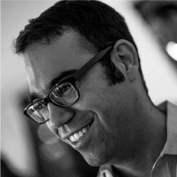
\includegraphics[height=2 cm]{kyle_cranmer.png}
\column{0.75\linewidth}
\begin{itemize}
\item Atlas physics research
\item RooStats and HistFactory, statistical procedures and Higgs combination
\item RECAST, \mbox{data preservation\hspace{-0.5 cm}} (NSF-funded DASPOS), Moore-Sloan Data Science Environment
\end{itemize}
\end{columns}
\end{columns}
\end{frame}

\end{document}
